

%%%%%%%%%%%%%%%%%%%%%%%%%%%%%%%%%%%%%%%%%%%%%%%%%%%%%%%%%%%%%%%%%%%%
%%%%%%%%%%%%%%%%%%%%%%%%%%%%%%%%%%%%%%%%%%%%%%%%%%%%%%%%%%%%%%%%%%%%
\chapter{Built-in applications}
\label{builtin}

% ==================================================================
\section{The Gazette}

% -----------------------------------------------------------------
\subsection{Overview}

The \wo{GAZETTE} is the observatory's logbook and calendar. It is a collection 
of \textbf{articles} in a relational DB table. An article is defined by: 
\begin{itemize}
\item a Start and an End timestamp,
\item a Category (from a predefined/editable list),
\item a list of Users (WebObs-registered and additional),
\item a Place,
\item a Subject.
\end{itemize}

The \wo{GAZETTE} has its own html interfaces for visualization and edition, implemented
in \wofile{CODE/cgi-bin/WebObs/Gazette.pm} and \wofile{CODE/cgi-bin/Gazette.pl} modules.

% -----------------------------------------------------------------
\subsection{Configuration}

The \wo{GAZETTE} is defined by a configuration file,
whose location is pointed to by the main WebObs configuration variable
GAZETTE\_CONF.

Among other parameters, GAZETTE\_CONF file points to the Gazette DataBase (DB\_NAME)
and the Gazette categories definitions (CATEGORIES\_FILE).

The \wo{GAZETTE} also uses the WebObs authorization mechanism with one resource associated to each 
category, plus one generic resource representing all categories. These resources
belong to the authorization 'misc' type (authmisc table), and are identified as  
"GAZETTE\textit{categoryKey}"  (eg. GAZETTEMissions, GAZETTEField). 

\begin{lstlisting}[title=\wofile{WEBOBS.rc} (excerpt)]
GAZETTE_CONF|${ROOT_CONF}/Gazette.rc
\end{lstlisting}

\lstinputlisting[title=\wofile{Gazette.rc}]{../../SETUP/CONF/Gazette.rc}

\lstinputlisting[title=\wofile{Gazette\_categories.conf}]{../../SETUP/CONF/Gazette_categories.conf}

The \wo{GAZETTE} also includes holidays definitions that can be adapted to any country using 
a specifications file pointed to by FILE\_DAYSOFF in the main WebObs configuration WEBOBS.rc .

\begin{lstlisting}[title=\wofile{WEBOBS.rc} (excerpt)]
FILE_DAYSOFF|${ROOT_CONF}/Holidays.conf
\end{lstlisting}

\lstinputlisting[title=\wofile{Holidays.conf} (example)]{../../SETUP/CONF/Holidays.conf}

% -----------------------------------------------------------------
\subsection{Display/Edit Gazette}

\wofile{CODE/cgi-bin/Gazette.pl} is the html interface used to request and display the Gazette. 
The greyed banner of the page is a selection form used to specify what and how Gazette articles should
be displayed: 
\begin{itemize}
\item What : Date or Date-range selection 
	\begin{itemize}
	\item \textbf{via a monthly calendar}
	\item \textbf{using predefined periods}
	\end{itemize}
\item What : Category and Filter
\item How : Presentation
	\begin{itemize}
	\item \textbf{Calendar}: a calendar-type weekly table,
	\item \textbf{List by categories}: a list sorted by categories,
	\item \textbf{List by date}: a list sorted by chronological start-date,
	\item \textbf{iCalendar}: iCal format text,
	\item \textbf{dump}: reserved for administrators, raw DB-table display
	\end{itemize}
\end{itemize}

The banner also displays a 'Create Article' button to trigger the edition of a new article.

Note: 'Event' category is not editable through html interface.

Developer's note: A Gazette display html code can also be imported into other pages using the WebObs/Gazette.pm 
Show function. See description in Gazette.pm perldoc and Welcome.pl page as an example.

% ==================================================================
\section{GRIDMAPS and LOCASTAT: maps of georeferenced nodes}

% -----------------------------------------------------------------
\subsection{Overview}

Any \wo{node} may be associated with a location with geographic coordinates. A \wo{proc} might use these coordinates for a specific processing, e.g. for tilt or gnss deformation modelling, or to produce dedicated maps. There is also two built-in applications that will use these coordinates: GRIDMAPS and LOCASTAT.

% -----------------------------------------------------------------
\subsection{GRIDMAPS}
\label{gridmaps}

When a \wo{node} is associated to a \wo{grid}, \webobs will automatically produce maps indicating these \wo{nodes}.

\begin{figure}
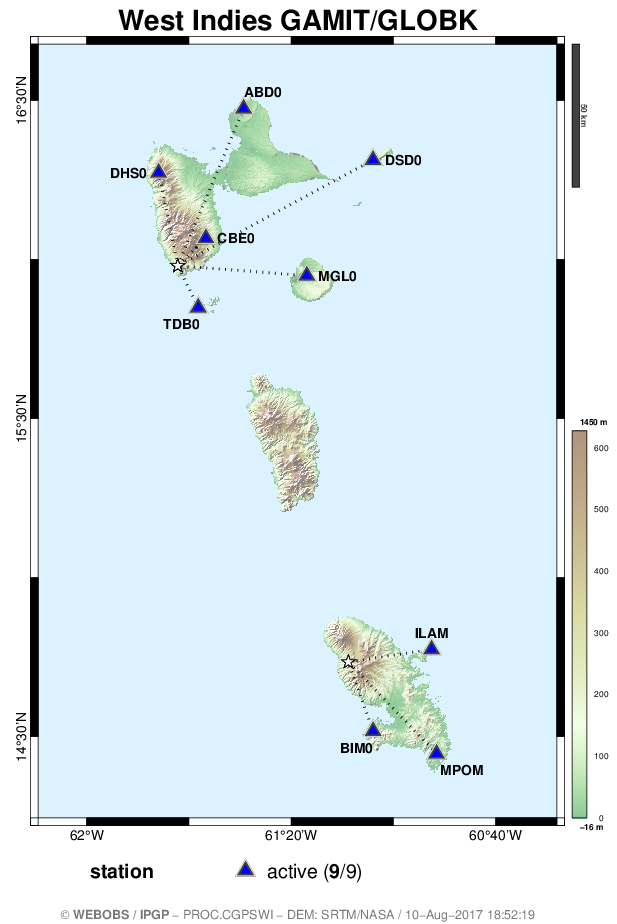
\includegraphics[height=.6\textwidth]{figures/PROC_CGPSWI_map.png}
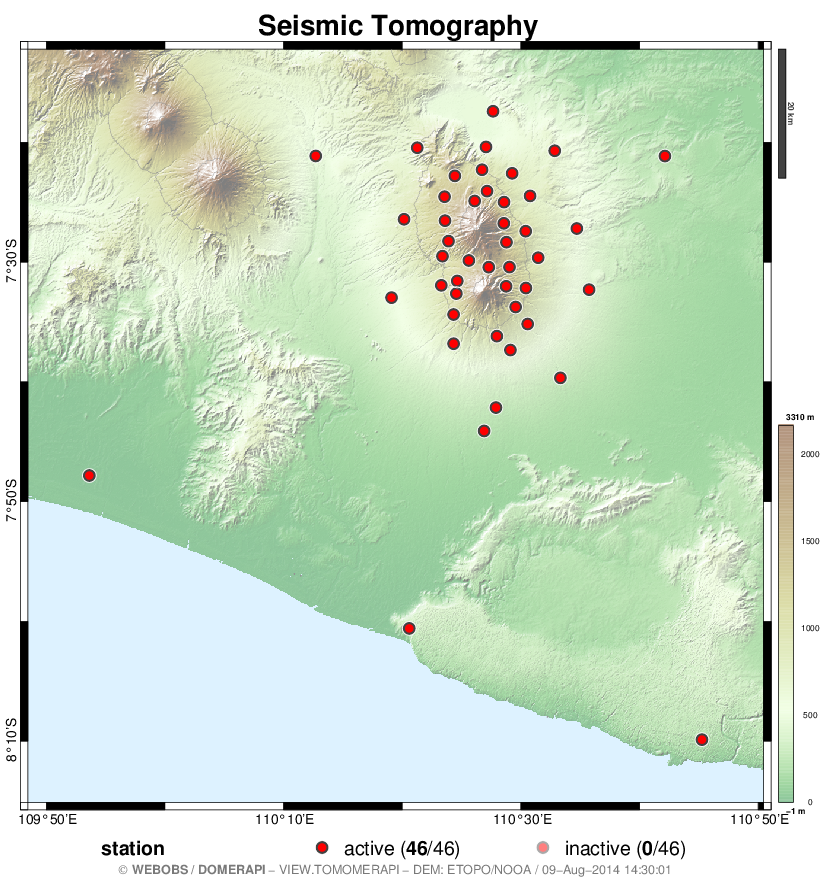
\includegraphics[height=.6\textwidth]{figures/VIEW_TOMOMERAPI_map.png}
\caption{Examples of GRID's maps created by GRIDMAPS.}
\end{figure}

% - - - - - - - - - - - - - - - - - - - - - - - - - - - - - - - - -
\subsubsection{Configuration}

Each \wo{grid} map is depending on two configuration files: one is common for all grids to define the basemap parameters:

\lstinputlisting[title=\wofile{GRIDMAPS.rc}]{../../SETUP/CONF/GRIDMAPS.rc}

and the other is the configuration file of the \wo{grid} itself to define the parameters associated to \wo{nodes} (see for example the \wo{view} example in section \ref{views}).

% - - - - - - - - - - - - - - - - - - - - - - - - - - - - - - - - -
\subsubsection{Activation}

GRIDMAPS is set by default when installing \webobs. It should be active at the first scheduler start. Parameters are as follows:

\begin{tabular}{rl}
\textbf{jid:}      & gridmaps \\
\textbf{res:}      & gridmaps \\
\textbf{xeq1:}     & \$WEBOBS\{JOB\_MCC\} gridmaps \\
\textbf{interval:} & 86400 \\
\textbf{logpath:}  & gridmaps \\
\textbf{valid:}    & Y \\
\end{tabular}

You may check if it runs correctly in the Scheduler Runs page (see Section \ref{scheduler}).


% -----------------------------------------------------------------
\subsection{LOCASTAT}
\label{locastat}

\begin{figure}
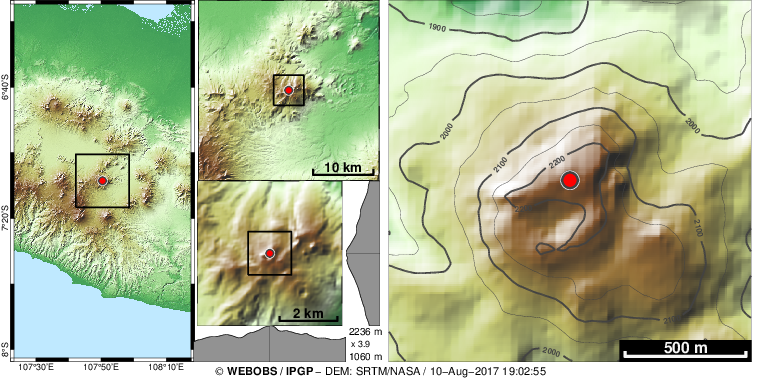
\includegraphics[width=\textwidth]{figures/IAIOBSPC01_map.png}
\caption{Example of NODE's map created by LOCASTAT.}
\end{figure}

The location map appears in each \wo{node} page if coordinates are defined. The map is automatically made and updated by LOCASTAT application. Maps are updated when the map timestamp is older than \wo{node}'s configuration file. So to force the update of a location map, you may modify any parameter in the \wo{node} configuration, typically the coordinates values or positioning date. 

The map contains 4 maps at different scales, all centered on the \wo{node} position, from left to right with a progressive zoom effect. Basemaps are built from the free worldwide topography data SRTM~\footnote{see \url{http://www2.jpl.nasa.gov/srtm/}} and specific colormap and rendering methods. It is possible to specify a user-defined DEM (Digital Elevation Model) for the highest resolution scale map (right frame).


\lstinputlisting[title=\wofile{LOCASTAT.rc}]{../../SETUP/CONF/LOCASTAT.rc}


% ==================================================================
\section{SEFRAN3/MC3: seismic chart and bulletin}

% -----------------------------------------------------------------
\subsection{Overview}

The SEFRAN3 is a graphical interface to operate seismic data flux, manual and semi-automatic detection of events, and earthquake catalog bulletin management.

The name ``SefraN'' is a contraction of \textit{Sefram Numérique}; it comes from a 70's paper strip-chart recording instrument from the French factory \textit{SEFRAM\textregistered}, used during decades in French observatories. Starting 2001, the system has been replaced by a numerical simulation using local data files archives in SUDS format. SEFRAN3 is the third version of SefraN which now uses data flow from SeedLink protocol.

A second tool called ``Main Courante'' hereafter named MC3, is a database of seismic events that is linked to SEFRAN3 interface and possibly to external earthquake catalogs like a local SeisComP3 or any FDSN-webservice compatible database like EMSC or USGS.

The SEFRAN3 works with a fixed selection of channels (up to 15) coming from a single server source, that will be displayed together as time series using 2 different time scales (normal and high) that simulate the paper speed. SEFRAN3 has 4 different GUI:
\begin{enumerate}

\item Main page showing hourly thumbnail images of seismic signals for a given period of time. Identified events are shown as overlaying colored tags. Bottom part of the page is showing realtime state of each channel with some statistics on the data quality. There is two display modes:
\begin{itemize}
\item real-time automatic refreshing page, for the last X hours/days of data;
\item any date selection for one or more days.
\end{itemize}

\item One hour display of full-resolution image in a wide window that can be spanned and scrolled through time.

\item A form showing a single event at high-speed time resolution of seismic signals, with possibility of editing data and submitting to the database.

\item A detailed table of events list with date selection, filters, and dynamic graphs.

\end{enumerate}

\textbf{Notice:} SEFRAN3 is using extensively the network connection (for data flux) and external programs like \wofile{arclink\_fetch} (from \textit{SeisComP3}), \wofile{slinktool} (from \textit{IRIS}) and \wofile{convert} (from \textit{ImageMagick}). If you experience any trouble, check first the network, the data availability on servers, and the third-party programs. You might add the variable \wokey{DEBUG|Y} in the configuration file to make the logs more verbose.

% -----------------------------------------------------------------
\subsection{SEFRAN3 installation}


\begin{figure}
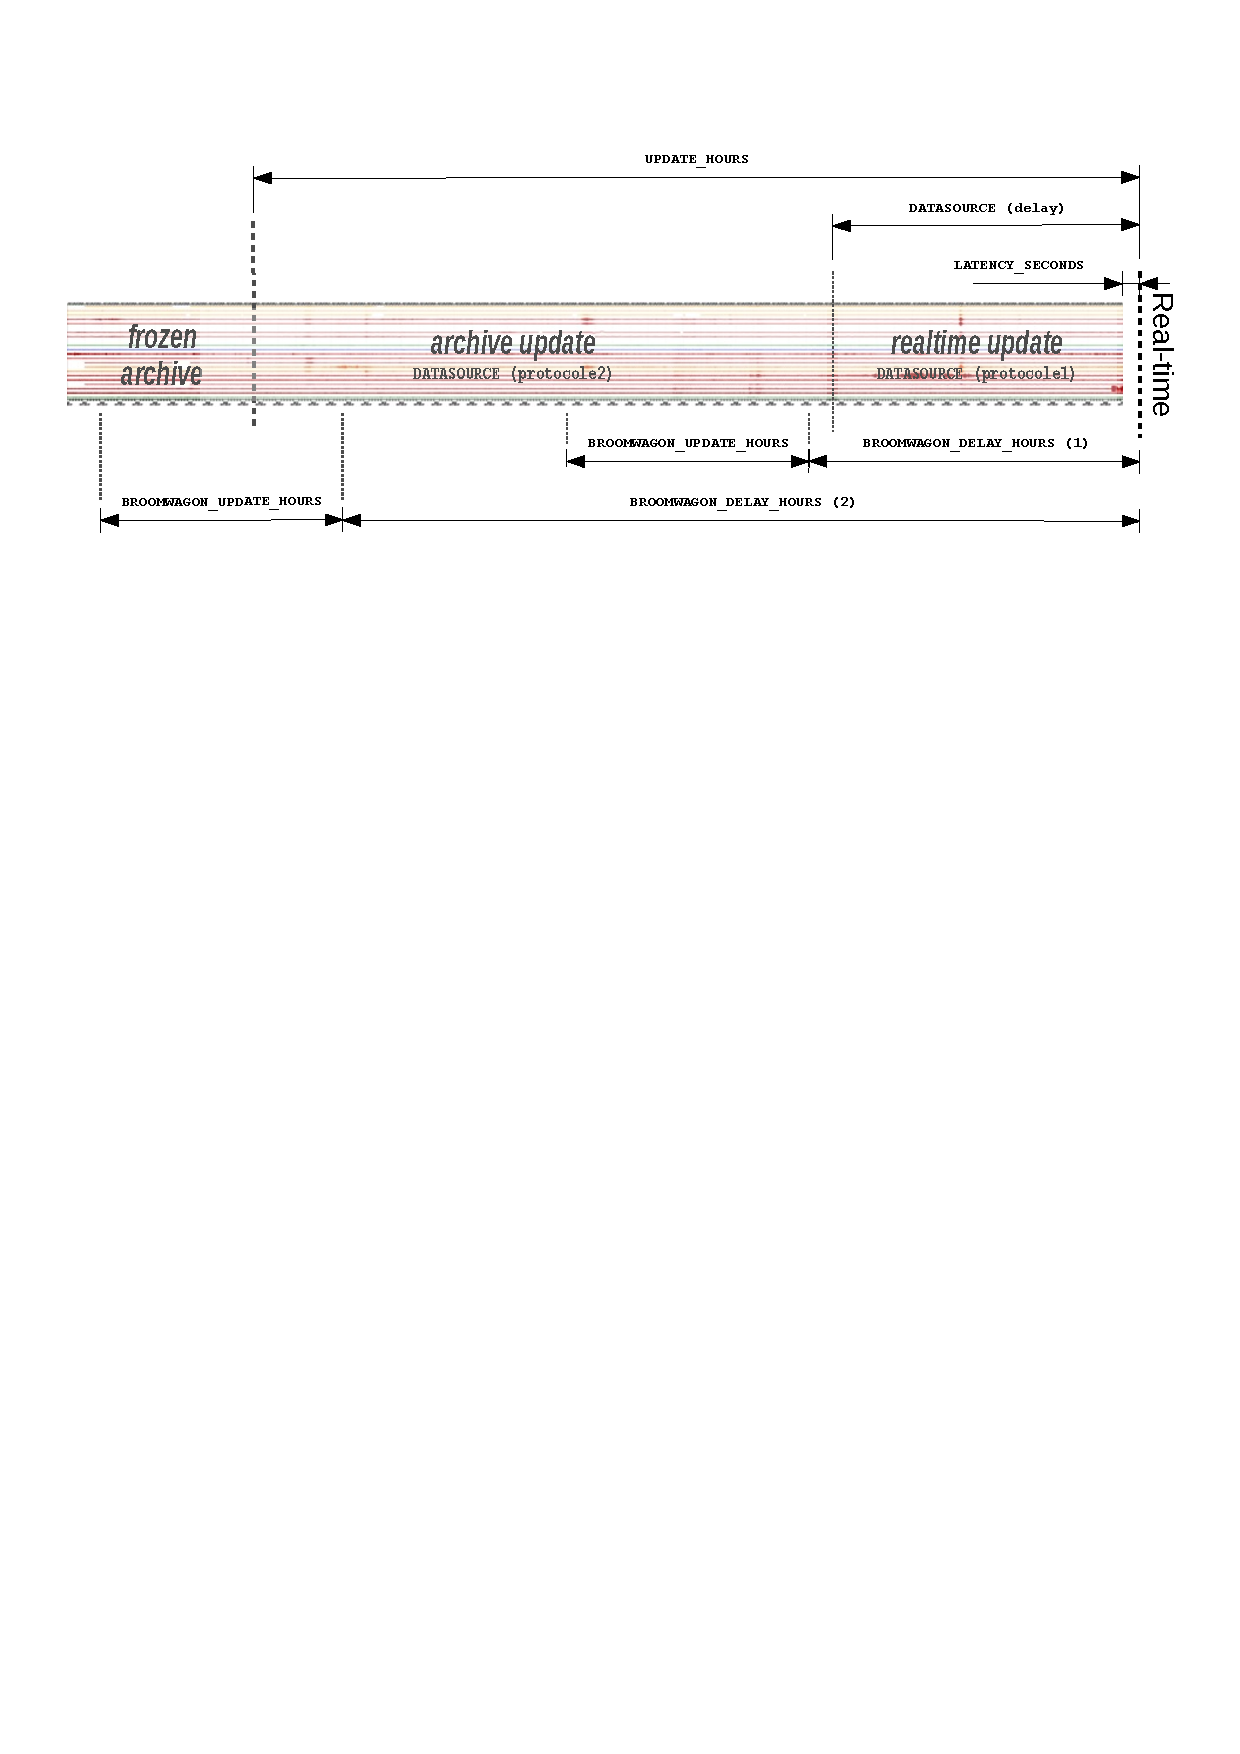
\includegraphics[width=\textwidth]{figures/sefran3_diagram.pdf}
\caption{Schematic diagram of SEFRAN3 main parameters.}
\label{sefran3_diagram}
\end{figure}

SEFRAN3 is based on 1-minute images of seismic traces. It works within a loop that will end after a minimum duration run. Each loop will scan the existing images on disk, and make new images (real-time first, then look at older periods for gaps) or update them using broom wagons that check the data completeness after some time delay. There is also a short delay of few seconds to take into account the data flux lateness from real-time, and a longer delay to switch from SeedLink data request (convenient for real-time data flux) to ArcLink data request (convenient for archived data). Figure \ref{sefran3_diagram} is a summary of main parameters.


% - - - - - - - - - - - - - - - - - - - - - - - - - - - - - - - - -
\subsubsection{Configuration files}

To configure a new SEFRAN3, copy the template files \wofile{SEFRAN3.conf} and \wofile{SEFRAN3\_Channels.conf} to, for example, \wofile{MYSEFRAN.conf} and \wofile{MYSEFRAN\_Channels.conf}.


\wofile{MYSEFRAN\_Channels.conf} file sets the channel list. Each channel is defined by its alias (a short code used for display), the stream string (used for the data request), the sensitivity factor (to convert counts to m/s), the filter (median, trend or spline removal), the peak-to-peak signal amplitude, and the color. A good conduct is to order the channels from North to South, and give different colors for specific regions. There is no limit to the number of channels, but a maximum of 15 channels is recommended for a normal screen resolution.

\wofile{MYSEFRAN.conf} file is the main configuration file. It defines a lot of things like output paths, server address and all parameters of graphical outputs and SEFRAN3 behavior.

\lstinputlisting[title=\wofile{SEFRAN3\_Channels.conf}]{../../SETUP/CONF/SEFRAN3_Channels.conf}

\lstinputlisting[title=\wofile{SEFRAN3.conf}]{../../SETUP/CONF/SEFRAN3.conf}


% - - - - - - - - - - - - - - - - - - - - - - - - - - - - - - - - -
\subsubsection{Activation}

To activate the SEFRAN3, add a new job in the scheduler, for example with following parameters:

\begin{tabular}{rl}
\textbf{jid:}      & mysefran \\
\textbf{res:}      & mysefran \\
\textbf{xeq1:}     & \$WEBOBS\{JOB\_MCC\} sefran3 \\
\textbf{xeq2:}     & MYSEFRAN \\
\textbf{interval:} & 600 \\
\textbf{logpath:}  & mysefran \\
\textbf{valid:}    & Y \\
\end{tabular}

After activation, check that it runs correctly in the Scheduler Runs page (see Section \ref{scheduler}).

To access the main SEFRAN3 page, use the following URL (can be set for instance in the menu bar):

\wocmd{/cgi-bin/sefran3.pl?header=1\&s3=MYSEFRAN}

Further options are available to access all display possibilities. See \wocmd{perldoc CODE/cgi-bin/sefran3.pl}.


% -----------------------------------------------------------------
\subsection{MC3 configuration}

\lstinputlisting[title=\wofile{MC3.conf}]{../../SETUP/CONF/MC3.conf}

\lstinputlisting[title=\wofile{MC3\_Codes.conf}]{../../SETUP/CONF/MC3_Codes.conf}

%\lstinputlisting[title=\wofile{MC3\_Headers.conf}]{../../SETUP/CONF/MC3_Headers.conf}

\lstinputlisting[title=\wofile{MC3\_Amplitudes.conf}]{../../SETUP/CONF/MC3_Amplitudes.conf}

\lstinputlisting[title=\wofile{MC3\_Durations.conf}]{../../SETUP/CONF/MC3_Durations.conf}


% -----------------------------------------------------------------
\subsection{Links with earthquake event catalogs}

% - - - - - - - - - - - - - - - - - - - - - - - - - - - - - - - - -
\subsubsection{SeisComP3}

% - - - - - - - - - - - - - - - - - - - - - - - - - - - - - - - - -
\subsubsection{EarthWorm}



% ==================================================================
\section{GENPLOT: generic time series}
\label{genplot}

% -----------------------------------------------------------------
\subsection{Overview}

GENPLOT is the default superproc to plot time series from any source of data, particularly the time series formats (see section \ref{timeseries}). GENPLOT is able to produce graphics and text outputs from data channels of associated NODES. All the outputs will be processed for a list of preset time scales, which can be any of the following:
\begin{itemize}
\item a fixed duration (expressed in hour, day, week, month or year) until the present time (moving window);
\item a window from a reference date until present time (extending window);
\item all available data.
\end{itemize}

GENPLOT will produce, for each time scale:
\begin{itemize}
\item one graph per \wo{node} showing separated subplot for each selected channel;
\item one summary graph combining all \wo{nodes} on each channel subplot using different colors.
\end{itemize}

The plotted channels for the per-node and summary graphs are both configurable
using respectively \wo{NODE\_CHANNELS} and \wo{SUMMARY\_CHANNELS}. Titles and
line and marker style can also be configured:
\begin{itemize}
\item set \wo{PERNODE\_TITLE} and/or \wo{SUMMARY\_TITLE} to customize the title;
\item set \wo{PERNODE\_LINESTYLE} and/or \wo{SUMMARY\_LINESTYLE} to a line specification string, a combination of two components:
	\begin{itemize}
		\item a line type (see possible values in table \ref{linestyle}),
		\item a marker symbol type (see possible values in table \ref{markertype}),
	\end{itemize}
 to choose between drawing markers and/or line and define their style; note you might specify a marker only with no line, then only the markers are plotted;
\item the line width and marker size can be different for each time scale using
  respectively \wo{LINEWIDTHLIST} and \wo{MARKERSIZELIST}, that should both
  define a size to use (in \texttt{pt}) for each of the timescales defined in
  \wo{TIMESCALELIST}, coma separated values;
\item colors are chosen automatically by the proc: for the summary graph it will be one color per node, for the per-node graph it will be one color per channel.
\end{itemize}

% -----------------------------------------------------------------
\subsection{Configuration}

Some parameter keys of GENPLOT are common for all \wo{procs} and \wo{grids} so are identical with the \wo{view} configuration (see section \ref{views}).

\lstinputlisting[title=\wofile{GENPLOT template}]{../../CODE/tplates/PROC.DEFAULT}

% - - - - - - - - - - - - - - - - - - - - - - - - - - - - - - - - -
\subsubsection{Time scales}



% ==================================================================
\section{HYPOMAP: Earthquake hypocenter maps from seismic catalog}

% -----------------------------------------------------------------
\subsection{Overview}

% -----------------------------------------------------------------
\subsection{Configuration}

Some parameter keys of HYPOMAP are common for all \wo{procs} and \wo{grids} so are identical with the \wo{view} configuration (see section \ref{views}).

\lstinputlisting[title=\wofile{HYPOMAP template}]{../../CODE/tplates/PROC.HYPOMAP}


% ==================================================================
\section{HELICORDER: Seismic helicorder}

% -----------------------------------------------------------------
\subsection{Overview}

% -----------------------------------------------------------------
\subsection{Configuration}

Some parameter keys of HELICORDER are common for all \wo{procs} and \wo{grids} so are identical with the \wo{view} configuration (see section \ref{views}).

\lstinputlisting[title=\wofile{HELICORDER template}]{../../CODE/tplates/PROC.HELICORDER}


% ==================================================================
\section{RSAM: Realtime Seismic Amplitude Measurement}

% -----------------------------------------------------------------
\subsection{Overview}

% -----------------------------------------------------------------
\subsection{Configuration}

Some parameter keys of RSAM are common for all \wo{procs} and \wo{grids} so are identical with the \wo{view} configuration (see section \ref{views}).

\lstinputlisting[title=\wofile{RSAM template}]{../../CODE/tplates/PROC.RSAM}


% ==================================================================
\section{GNSS: GPS time series, vectors and modelling}

% -----------------------------------------------------------------
\subsection{Overview}

% -----------------------------------------------------------------
\subsection{Configuration}

Some parameter keys of GNSS are common for all \wo{procs} and \wo{grids} so are identical with the \wo{view} configuration (see section \ref{views}).

\lstinputlisting[title=\wofile{GNSS template}]{../../CODE/tplates/PROC.GNSS}


% ==================================================================
\section{EXTENSO: Extensometry time series and vectors}

% -----------------------------------------------------------------
\subsection{Overview}

% -----------------------------------------------------------------
\subsection{Configuration}

Some parameter keys of EXTENSO are common for all \wo{procs} and \wo{grids} so are identical with the \wo{view} configuration (see section \ref{views}).

\lstinputlisting[title=\wofile{EXTENSO template}]{../../CODE/tplates/PROC.EXTENSO}


% ==================================================================
\section{TILT: Tiltmetry time series, vectors and modelling}

% -----------------------------------------------------------------
\subsection{Overview}

% -----------------------------------------------------------------
\subsection{Configuration}

Some parameter keys of TILT are common for all \wo{procs} and \wo{grids} so are identical with the \wo{view} configuration (see section \ref{views}).

\lstinputlisting[title=\wofile{TILT template}]{../../CODE/tplates/PROC.TILT}


% ==================================================================
\section{METEO: meteorological time series}

% -----------------------------------------------------------------
\subsection{Overview}

% -----------------------------------------------------------------
\subsection{Configuration}

Some parameter keys of METEO are common for all \wo{procs} and \wo{grids} so are identical with the \wo{view} configuration (see section \ref{views}).

\lstinputlisting[title=\wofile{METEO template}]{../../CODE/tplates/PROC.METEO}


% ==================================================================
\section{WATERS: chemical analysis}

% -----------------------------------------------------------------
\subsection{Overview}

% -----------------------------------------------------------------
\subsection{Configuration}

Some parameter keys of WATERS are common for all \wo{procs} and \wo{grids} so are identical with the \wo{view} configuration (see section \ref{views}).

\lstinputlisting[title=\wofile{WATERS template}]{../../CODE/tplates/PROC.WATERS}



% ==================================================================
\section{PROCS graph and data request}

% -----------------------------------------------------------------
\subsection{Overview}

A dedicated form \wocmd{/cgi-bin/formREQ.pl} allows to make user request to get any outputs (graphs and data) from PROCS sharing the same set of time span and parameters, mostly independent from the SCHEDULER's jobs. The identified USER has to be authorized for reading on the PROC to perform a request on it.

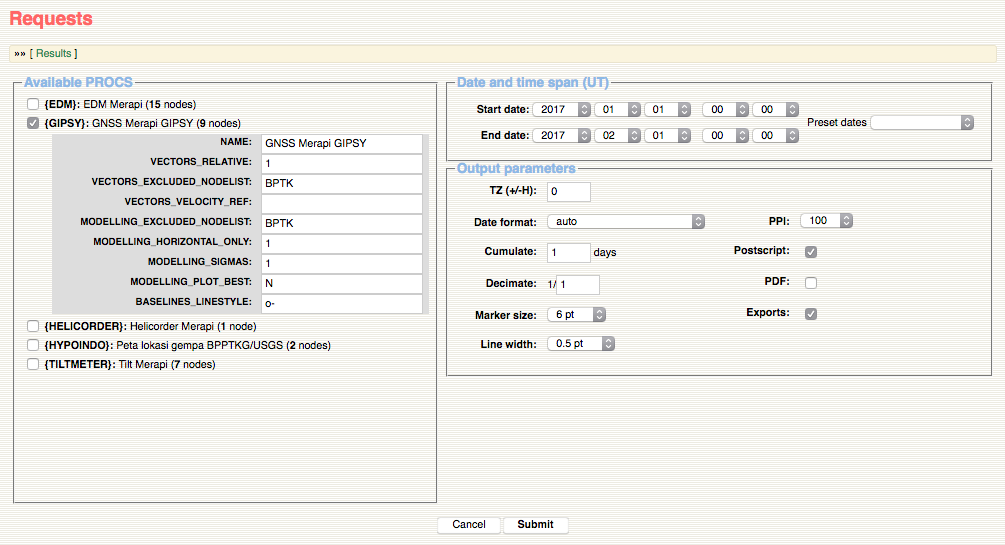
\includegraphics[width=\textwidth]{figures/formREQ.png}

% -----------------------------------------------------------------
\subsection{Description}

The form presents a list of available PROCS with empty check boxes. One or more PROCS can be selected, in that case a parameter list might appear for each of selected PROC, allowing the user to change the values. Please note there is no validity check of the values so a request may fail in case of invalid fields.

The main parameter to define is the date and time span: \textbf{Start date} and \textbf{End date} with time. Default is the last full month. A list of preset dates is also available. The date and time must be in UT. 

Also some output parameters can be defined:
\begin{itemize}
\item \textbf{TZ:} the output time zone, in hours. Will affect graphs and data exports.
\item \textbf{Date format:} the format of dates for time series plots axis ticks label.
\item \textbf{Cumulate:} time for cumulating data (when cumulative allowed in the PROC), in day. Use fraction or any arithmetic formula if needed.
\item \textbf{Decimate:} number of sample for decimation of the raw data (time series).
\item \textbf{Marker size:} maker size in points (if the PROC uses markers).
\item \textbf{Line width:} line width in points (if the PROC uses lines).
\item \textbf{PPI:} resolution for PNG output images, in pixel per inch.
\item \textbf{Postscript:} outputs the EPS vector graphic images (default is cheched).
\item \textbf{PDF:} outputs a PDF version of images.
\item \textbf{Exports:} outputs data (text files or others depending on the PROC).
\end{itemize}

After submit the request, each of the PROC will be submitted to SCHEDULER as specific jobs. The name of the job is made from date and time of the request, hostname and user login name.

The run of each PROC can be followed on the scheduler runs page. If a job ends with success, a notification email is sent to the user through the POSTBOARD. The email provides two links: a first to access the request results (graphs and exports) through a web interface similar to the routine PROC graphs. The second link allows to download a .tgz archive containing all images and files of the request.

A dedicated page is also available to access request results: \wocmd{/cgi-bin/showREQ.pl}. The page will show the user's requests and results (if the request job has ended successfully), or all the existing requests for ADMIN users.


% -----------------------------------------------------------------
\subsection{Configuration}

\begin{lstlisting}[title=\wofile{PROC.conf} (excerpt)]
SUBMIT_COMMAND|$WEBOBS{JOB_MCC} genplot $SELFREF -
SUBMIT_RESOURCE|myproc
REQUEST_KEYLIST|NAME,SUMMARY_RELATIVE,PERNODE_LINESTYLE
\end{lstlisting}

The request form displays any PROC containing a not-empty \wokey{SUBMIT\_COMMAND} parameter in its configuration. This parameter is the routine execution command line, ie. equivalent to the value of a XEQ1 in the SCHEDULER (see scheduler.pl doc) and, as such,
supporting \wo{\$WEBOBS} parameters substitution.

The \wokey{SUBMIT\_RESOURCE} is the optional routine execution mutex name (process lock) of as defined in SCHEDULER if the PROC is one of the routine jobs. This is to avoid possible conflicts of simultaneous runs.

Optionally, the \wokey{REQUEST\_KEYLIST} parameter is used to specify a list of comma-separated keys of existing parameters, that will be
presented to the user so that (s)he will have a chance to overwrite corresponding values for request execution.

The user defined output parameters \textbf{Date format}, \textbf{Cumulate}, \textbf{Decimate}, \textbf{Marker size} and \textbf{Line width} correspond to table values \wokey{DATESTRLIST}, \wokey{CUMULATELIST}, \wokey{DECIMATELIST}, \wokey{MARKERSIZELIST} and \wokey{LINEWIDTHLIST}, respectively.

The list of available preset values for PPI resolution, marker size and line width can be defined in \wofile{WEBOBS.rc} :

\begin{lstlisting}[title=\wofile{WEBOBS.rc} (excerpt)]
REQ_PPI_LIST|75,100,150,300,600
REQ_MARKERSIZE_LIST|1,2,4,6,10,15,20
REQ_LINEWIDTH_LIST|0.1,0.25,0.5,1,1.5,2,3
\end{lstlisting}

To use the notification email facility, POSTBOARD must be running, and the special event \textbf{formreq.} must be defined and valid (see \webobs Users Manager page).



% ==================================================================
\section{Data formats available for PROCS}

Formats are defined for a whole PROC in the \wokey{RAWFORMAT} PROC's variable, or for individual NODE in the \wokey{RAWFORMAT} NODE's parameter which overwrites the PROC value. The \wokey{RAWDATA} PROC's variable can be defined for all associated NODES, and any individual NODE's \wokey{RAWDATA} may overwrite it. A special variable \wocmd{\$FID} might be used and will be replaced by each NODE's value. For most of the formats, the Calibration File of each associated NODE will define the list of available channels and associated parameters.

See the source codes \wofile{CODE/matlab/readfmtdata.m} help for more details.

% -----------------------------------------------------------------
\subsection{Waveforms formats}

These formats are standards in seismology for waveforms data, but they are also used for other types of geophysical sensors. The standards use local files in specific format or dedicated protocol request from distant servers. Particularly, the full channel stream must be defined for each NODE, i.e.:

\begin{tabular}{ccl}
NET & network code & \wokey{FDSN\_NETWORK\_CODE} NODE's parameter\\
STA & station code & \wokey{FID} NODE's parameter\\
CHA & channel code & calibration file ``Chan. Code'' channel parameter\\
LOC & location code & calibration file ``LC'' channel parameter\\
\end{tabular}


% - - - - - - - - - - - - - - - - - - - - - - - - - - - - - - - - -
\subsubsection{\{miniseed\}: miniSEED files}
\label{miniseed}

Single of multiple local files in miniSEED format. \wokey{RAWDATA} defines the filename(s) using standard bash syntax (accepts wildcards). Some limitations may apply due to bash line size limit.


% - - - - - - - - - - - - - - - - - - - - - - - - - - - - - - - - -
\subsubsection{\{seedlink\}: SeedLink request}
\label{seedlink}

SeedLink protocol request from a distant or local server. \wokey{RAWDATA} defines the server with \wocmd{host:port}. The format uses external program \wocmd{slinktool} defined by the \wofile{WEBOBS.rc} \wokey{SLINKTOOL\_PRGM} parameter. \wokey{DATALINK\_DELAY\_SECONDS} defines the delay in seconds from real-time for the last data.


% - - - - - - - - - - - - - - - - - - - - - - - - - - - - - - - - -
\subsubsection{\{arclink\}: SeisComP3 ArcLink request}
\label{arclink}

ArcLink protocol request from a distant or local server. \wokey{RAWDATA} defines the server with \wocmd{host:port}. Optional parameter \wokey{ARCLINK\_USER} can be defined (default user is 'wo'). The format uses external program \wocmd{arclink\_fetch} defined by the \wofile{WEBOBS.rc} \wokey{ARCLINKFETCH\_PRGM} parameter.

% - - - - - - - - - - - - - - - - - - - - - - - - - - - - - - - - -
\subsubsection{\{combined\}: SeisComP3 combined SeedLink/ArcLink request}

The combined format will use SeedLink protocol for recent data and ArcLink protocol for data older than a delay. \wokey{RAWDATA} must contain the string \wocmd{seedlinkhost:seedlinkport;arclinkhost:arclinkport;delayhours}. It will use both external programs defined in \wofile{WEBOBS.rc} \wokey{SLINKTOOL\_PRGM} and \wokey{ARCLINKFETCH\_PRGM} parameters.

% - - - - - - - - - - - - - - - - - - - - - - - - - - - - - - - - -
\subsubsection{\{fdsnws-dataselect\}: FDSN web-service dataselect request}

Distant waveform request using the FDSN web-service protocol available at most of seismological data centers. \wokey{RAWDATA} must contain the base URL, for example: \wocmd{http://service.iris.edu/fdsnws/dataselect/1/query?} for IRIS.

% - - - - - - - - - - - - - - - - - - - - - - - - - - - - - - - - -
\subsubsection{\{winston\}: EarthWorm Winston wave server request}

EarthWorm Winston wave server (WWS) protocol request from a distant or local server. \wokey{RAWDATA} defines the server with \wocmd{host:port}.


% -----------------------------------------------------------------
\subsection{Generic time series}
\label{timeseries}

These formats will return time series of data channels, like the waveform formats do but usually the data sampling frequency is lower than for seismic waveforms, so it can be managed using data files stored in local directories. Number of channels depends on the data and can be selected and calibrated using the NODE's calibration file.

% - - - - - - - - - - - - - - - - - - - - - - - - - - - - - - - - -
\subsubsection{\{ascii\}: Generic ASCII text files}

Attempt to read generic text files with regular data columns. \wokey{RAWDATA} contains the full path and filename(s) using bash wildcard facilities. The data files must be organized as regular columns of numbers (strings will produce a column of NaN), any separator character, and the date and time must be defined as 3 (year, month, day) or 6 columns (year, month, day, hour, minute, second) at some place (default is the 6 first columns). If there is no calibration file for a NODE, the header line will be used to get the channel names.

For this format you may define optional additional \wokey{FID\_*} keys for each NODE to specify the format:

\begin{tabular}{rl}
\wokey{FID\_FS} & field separator character (default is semicolumn),\\
\wokey{FID\_TIMECOLS} & index vector of columns defining date\&time in order: year month day hour minute second,\\
\wokey{FID\_NF} & number of data columns in the file, considering all non-numeric as separator (default is automatic),\\
\wokey{FID\_HEADERLINES} & number of header lines (default is 1).
\end{tabular}


\begin{lstlisting}[language={},title=Generic ASCII format example 1: time + data channels 1 to 3.]
               Date;                   P_0;                 SO2_0;                 H2S_0;
06/06/2017 18:00:00;            752.579529;             -0.061299;             -0.031172;
06/06/2017 18:00:09;            724.445852;             -0.071515;             -0.024938;
\end{lstlisting}

\begin{lstlisting}[title=\wokey{FID\_*} parameters to read example 1 file.]
FID_FS|;
FID_TIMECOLS|3,2,1,4,5,6
FID_NF|9
FID_HEADERLINES|1
\end{lstlisting}


\begin{lstlisting}[language={},title=Generic ASCII format example 2: data channel 1 (all NaN) + time + data channels 2 to 4.]
VMAB    01/01/12        06:20:11        132     338     40.6
VMAB    01/01/12        06:40:11        135     337     40.7
VMAB    01/01/12        07:00:11        133     336     40.6
\end{lstlisting}


\begin{lstlisting}[title=\wokey{FID\_*} parameters to read example 2 file.]
FID_FS|\t
FID_TIMECOLS|4,3,2,5,6,7
FID_NF|10
FID_HEADERLINES|0
\end{lstlisting}


% - - - - - - - - - - - - - - - - - - - - - - - - - - - - - - - - -
\subsubsection{\{sql-table\}: SQL-table request}

Request to a SQL database using external program \wocmd{mysql}. \wokey{RAWDATA} must contain the full command that will return the data in the text format \wocmd{yyyy-mm-dd HH:MM:SS data1 data2 data3 ...}. The command must include two variables \wocmd{\$date1} and \wocmd{\$date2} that will be replaced by the timespan request. Example:

\wocmd{mysql -h host -u user -ppasswd -Ddatabase -N -B -e 'SELECT time,data1,data2,data3 from \$FID WHERE time between "\$date1" and "\$date2";'}

will make a request from the \wocmd{database} at server \wocmd{host} on the table \wocmd{\$FID} and return timestamp and data columns. The calibration file must define these 3 channels in that order.

% - - - - - - - - - - - - - - - - - - - - - - - - - - - - - - - - -
\subsubsection{\{cr10xasc\}: Campbell Scientific CR10X ASCII files}

Daily data files from data loggers CR10X archived in a specific directory structure. \wokey{RAWDATA} contains the main directory path, in which files are stored in the following subpath and name: \wocmd{FID/YYYY/YYYYMMDD.DAT}. Each file has the data format: \wocmd{PRGM,yyyy,doy,HM,data1,data2, ... ,dataN}, where \wocmd{PRGM} is the program number, \wocmd{yyyy} the 4-digit year, \wocmd{doy} the day of the year (ordinal day), \wocmd{HM} the hour and minute with leading blanks, and the data.

\begin{lstlisting}[language={},title=Campbell CR10X format example]
121,2013,365,2340,8.6971,-20.168,0,91.3,22.48,0,826.42,12.514,99999,0,0
121,2013,365,2350,8.7294,-20.016,0,88.4,20.02,0,826.43,12.521,99999,0,0
\end{lstlisting}


% - - - - - - - - - - - - - - - - - - - - - - - - - - - - - - - - -
\subsubsection{\{t0a5\}: Campbell Scientific T0A5 ASCII files}

Daily data files from Campbell Scientific data loggers in the T0A5 output format, archived in a specific directory structure. \wokey{RAWDATA} contains the main directory path, in which files are stored in the following subpath and name: \wocmd{FID/YYYY/FIDYYYYDDD.DAT}. Each file has the data format: \wocmd{"yyyy-mm-dd HH:MM:SS",data1,data2, ... ,dataN}.

\begin{lstlisting}[language={},title=Campbell T0A5 format example]
"2014-01-11 00:00:00",68148,12.1,16.07,15.29,100,938,0.02,0.02,0,7.875425,98.67353,10.86884,0,0,0,0,0,0,0,0
"2014-01-11 00:10:00",68149,12.1,15.96,14.76,100,938,0.021,0.021,0,7.200668,101.9742,11.35311,0,0,0,0,0,0,0,0
\end{lstlisting}


% - - - - - - - - - - - - - - - - - - - - - - - - - - - - - - - - -
\subsubsection{\{porkyasc\}: USGS Porky ASCII files}

Daily data files from USGS Porky data systems, archived in a specific directory structure. \wokey{RAWDATA} contains the main directory path, in which files are stored in the following subpath and name: \wocmd{FID/YYYY/YYYYMMDD.DAT}. Each file has the data format: \wocmd{DD-MMM-YYYY HH:MM data1 data2 ... dataN}.

\begin{lstlisting}[language={},title=USGS Porky format example]
01-JAN-2014 00:00  00000  00029  00013  03181  00001 -00998 -00998 -00998
01-JAN-2014 00:05  00001  00040  00010  03182  00001 -00998 -00998 -00998
\end{lstlisting}

% -----------------------------------------------------------------
\subsection{Quakes catalogs}

These are specific formats for PROCS dedicated to earthquake catalogs. These formats returns a list of event with preset channels, like Latitude, Longitude, Depth, Magnitude, etc... There is no calibration file (if it exists it will be ignored). It is possible to link this format with a Main Courante (MC3) database using the NODE's \wokey{FID\_MC3} with the MC3 name. In that case some information from MC3 might be associated to identified events.

An other specificity of these formats is that all catalogs from different associated NODES will be concatenated in a single data matrix. This allows to merge for instance, a distance worldwide catalog like USGS (for large earthquakes), a local catalog from a local network, and an historical catalog in an old-fashion file format.

% - - - - - - - - - - - - - - - - - - - - - - - - - - - - - - - - -
\subsubsection{\{hyp71sum2k\}: Quake Hypo71 summary lines year 2000 compatible}

Single file in the HYPO71 ASCII format identified by \wokey{RAWDATA} with full filename and path. The standard format is completed by two last columns: \wocmd{SCode} for a 5-letter identification code, and \wocmd{File} for the waveform filename. Note the file is column formatted, without any delimiter, there is no leading zeros but blanks, and the longitude value is positive towards the West.

\begin{lstlisting}[title=HYPO71 format example]
#   DATE ORIGIN     LAT_N     LON_W     DEPTH    MAG NO GAP DMIN  RMS  ERH  ERZ Q  SCode File
18430208 1440 00.00 16-44.00  61-10.00 000.00   8.00 00 000 00.0 0.00 00.0 00.0 0  TE9GM
20141005 1819 07.34 14-48.70  61-10.33  -0.24 D 1.52  8 166  0.3 0.26  0.6  0.8 C  EB1   20141005_181900.mq0
\end{lstlisting}


% - - - - - - - - - - - - - - - - - - - - - - - - - - - - - - - - -
\subsubsection{\{fdsnws-event\}: Quake FDSN WebServices event request}

Distant event data request using the FDSN web-service protocol available at most of seismological data centers. It accepts the QuakeML 1.2 format only. \wokey{RAWDATA} must contain the base URL, for example: \wocmd{http://service.iris.edu/fdsnws/event/1/query?} for IRIS.


% - - - - - - - - - - - - - - - - - - - - - - - - - - - - - - - - -
\subsubsection{\{scevtlog-xml\}: Quake SeisComP3-xml files}

Reads a files architecture created by the SeisComP3 scevtlog module. \wokey{RAWDATA} defines the path root where events are stored in a subdirectory structure as \wofile{YYYY/MM/DD/eventID/eventID.last.xml} in the SC3ML format.


% -----------------------------------------------------------------
\subsection{GNSS solutions}

These are specific formats for PROCS dedicated to positioning data from GNSS (Global Network Satellite Systems) like GPS or GLONASS. These formats returns preset channels: Eastern, Northern, Vertical and Orbit type.

% - - - - - - - - - - - - - - - - - - - - - - - - - - - - - - - - -
\subsubsection{\{gipsy-tdp\}: JPL GIPSY-OASIS TDP files}

TDP (Time Dependant Parameter) files results of the JPL GIPSY-OASIS processing in IRTF. The format uses only the position part of the data: \wocmd{Time   Dinit   Dfinal error STA c ssss} where Time is GPS date in seconds past J2000, \wocmd{c} is the component in geocentric referential, \wocmd{ssss} the station name. \wokey{P.RAWDATA} contains the path root directory where daily solutions files are stores in a subdirectory structure as \wofile{FID/YYYY/FID/YYYY-MM-DD.FID.tdp*}.

\begin{lstlisting}[language={},title=GIPSY-OASIS TDP format example]
 476712000.0000   1797.11460400000       1797.11463384421      9.751E-07  STA Z   ABD0
 476712000.0000  -5375.91966100000      -5375.91974126823      2.297E-06  STA Y   ABD0
 476712000.0000   2920.34971800000       2920.34975977472      1.377E-06  STA X   ABD0
\end{lstlisting}


% - - - - - - - - - - - - - - - - - - - - - - - - - - - - - - - - -
\subsubsection{\{globkval\}: MIT GAMIT-GLOBK VAL files}

Single file output of Gamit-GlobK processing in ITRF referencing. \wokey{P.RAWDATA} defines the full path filename of the .VAL result file which contains solution timeseries for each component and each station.

\begin{lstlisting}[language={},title=GAMIT-GLOBK VAL format example]
 Combination of ALL networks
ILAM_GPS to E Solution  1 +  32197594.810 m

 2012 12 19 11 59  32197594.80990    0.00626   -0.00183   0.00626
 2012 12 20 11 59  32197594.81087    0.00433   -0.00090   0.00433
 ...
 2013 12 17 11 59  32197594.81866    0.00519   -0.00799   0.00519

Wmean   32197594.8184 m +- 0.0003 from  340 data. WRMS   5.2 mm, NRMS  1.19
Slope    15.01 +-     0.84 mm/yr, WRMS   3.1 mm, NRMS  0.70, dur  0.99 <> 2013.41 yr

 Combination of ALL networks
ILAM_GPS to U Solution  1 +        -0.750 m

 2012 12 19 11 59        -0.74977    0.01910    0.01410   0.01910
 2012 12 20 11 59        -0.74919    0.01048    0.01471   0.01048
 ...
 2013 12 17 11 59        -0.80060    0.01370   -0.02614   0.01370

Wmean         -0.7686 m +- 0.0006 from  340 data. WRMS   9.3 mm, NRMS  0.82
Slope   -10.66 +-     2.20 mm/yr, WRMS   8.8 mm, NRMS  0.78, dur  0.99 <> 2013.41 yr
\end{lstlisting}


% -----------------------------------------------------------------
\subsection{Other specific formats}

These formats are basically time series but the channels are predefined.

% - - - - - - - - - - - - - - - - - - - - - - - - - - - - - - - - -
\subsubsection{\{teqc-qc\}: TEQC Rinex quality check}

% - - - - - - - - - - - - - - - - - - - - - - - - - - - - - - - - -
\subsubsection{\{naqs-soh\}: NAQS State of Health}

% - - - - - - - - - - - - - - - - - - - - - - - - - - - - - - - - -
\subsubsection{\{wodbform\}: WebObs database forms}

This format is not selectable. It becomes active automatically when a PROC is associated to a FORM and its specific database. In that case the data columns are determined by the FORM type.
